%% The ``\maketitle'' command must be the first command after the
%% ``\begin{document}'' command. It prepares and prints the title block.

%% the only exception to this rule is the \firstsection command
\firstsection{Introduction}

\maketitle
HDI is an useful index that shows how much a country has been developed over a year in term of human development. The HDI value is calculated based on four dimensions: life expectancy at birth, expected years of schooling, mean years of schooling, and GNI per capita~\cite{HDIinfo}.
There are several existing HDI visualization tools that allow user to view the dataset in a non-interactive way. For example, UNDP has a line chart as shown in Figure~\ref{fig:undp}. The x-axis indicates years, and the y-axis indicates HDI values. Each line represents one country that users can hover on to see the HDI value. The users can view the common trend for all the countries and find a country with the highest or lowest HDI value for a given year. However, there is no much information they can retrieve from the middle range of data where many lines congest together.

In this project, we are interested in making a better HDI visualization to address the limitation of existing visualization. For example, the chart in Figure~\ref{fig:undp} does not have a way for users to select a country. Another major visualization for HDI is Visualizing Human Development Index 2013 from Amazon AWS as shown in Figure \ref{fig:amazon}, providing four line charts for HDI components and a color map showing different HDI values. Users are able to hover on the map or the line to see the corresponding country highlighted. It also includes a population chart for viewing how the population is distributed among different HDI values.  The comparison view between the map and the graphs provides more information than the single line chart from UNDP. However, it did not provide any filtering functionality if the users only want to view countries with high HDI. It is also be hard to find a country as well if the users do not know where the country is located on the map. Our visualization can provide users more functionality to interact with the visualization so that they can easily find information they need.
\begin{figure}[t]
    \centering
    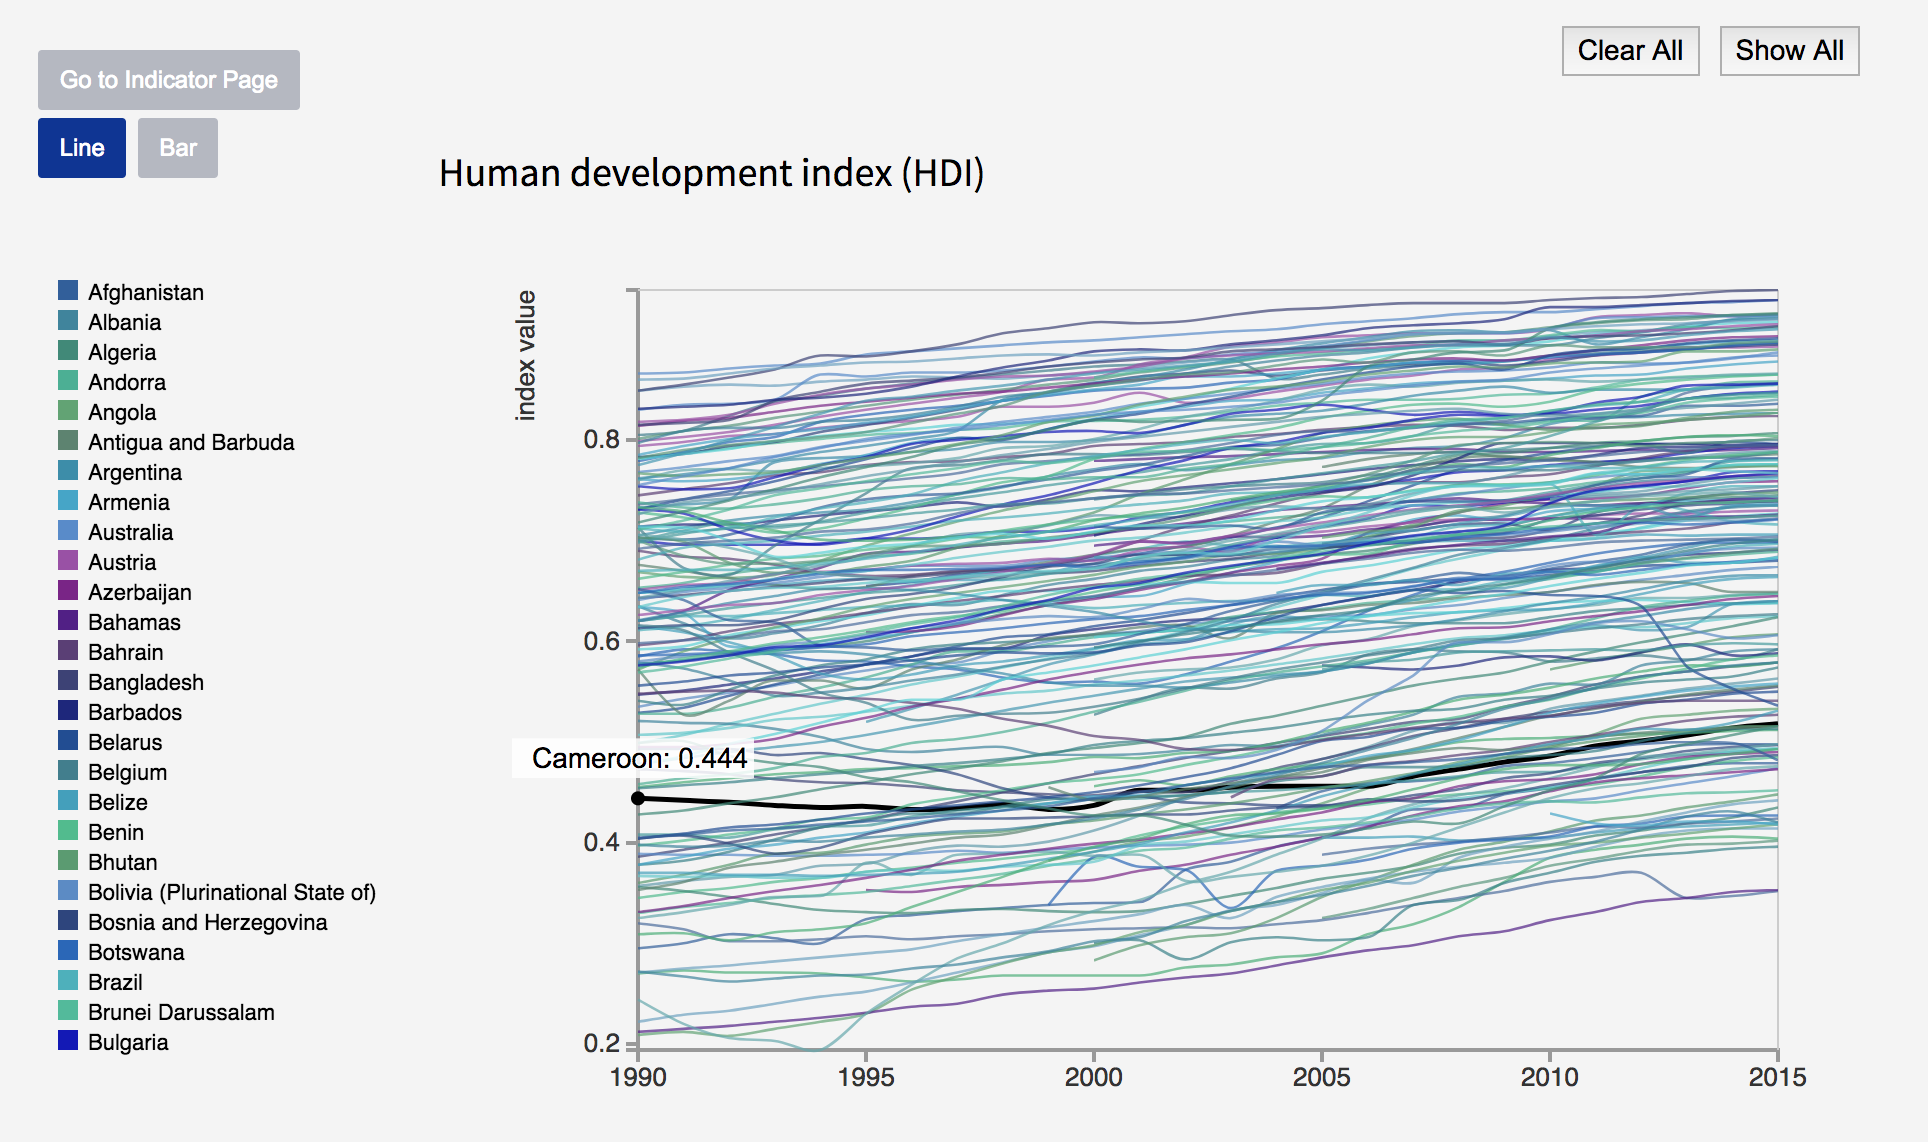
\includegraphics[width=0.4\textwidth]{undp}
    \caption{Line chart map from UNDP~\cite{UNDPlinechart}}
    \label{fig:undp}
\end{figure}
\begin{figure}[t]
    \centering
    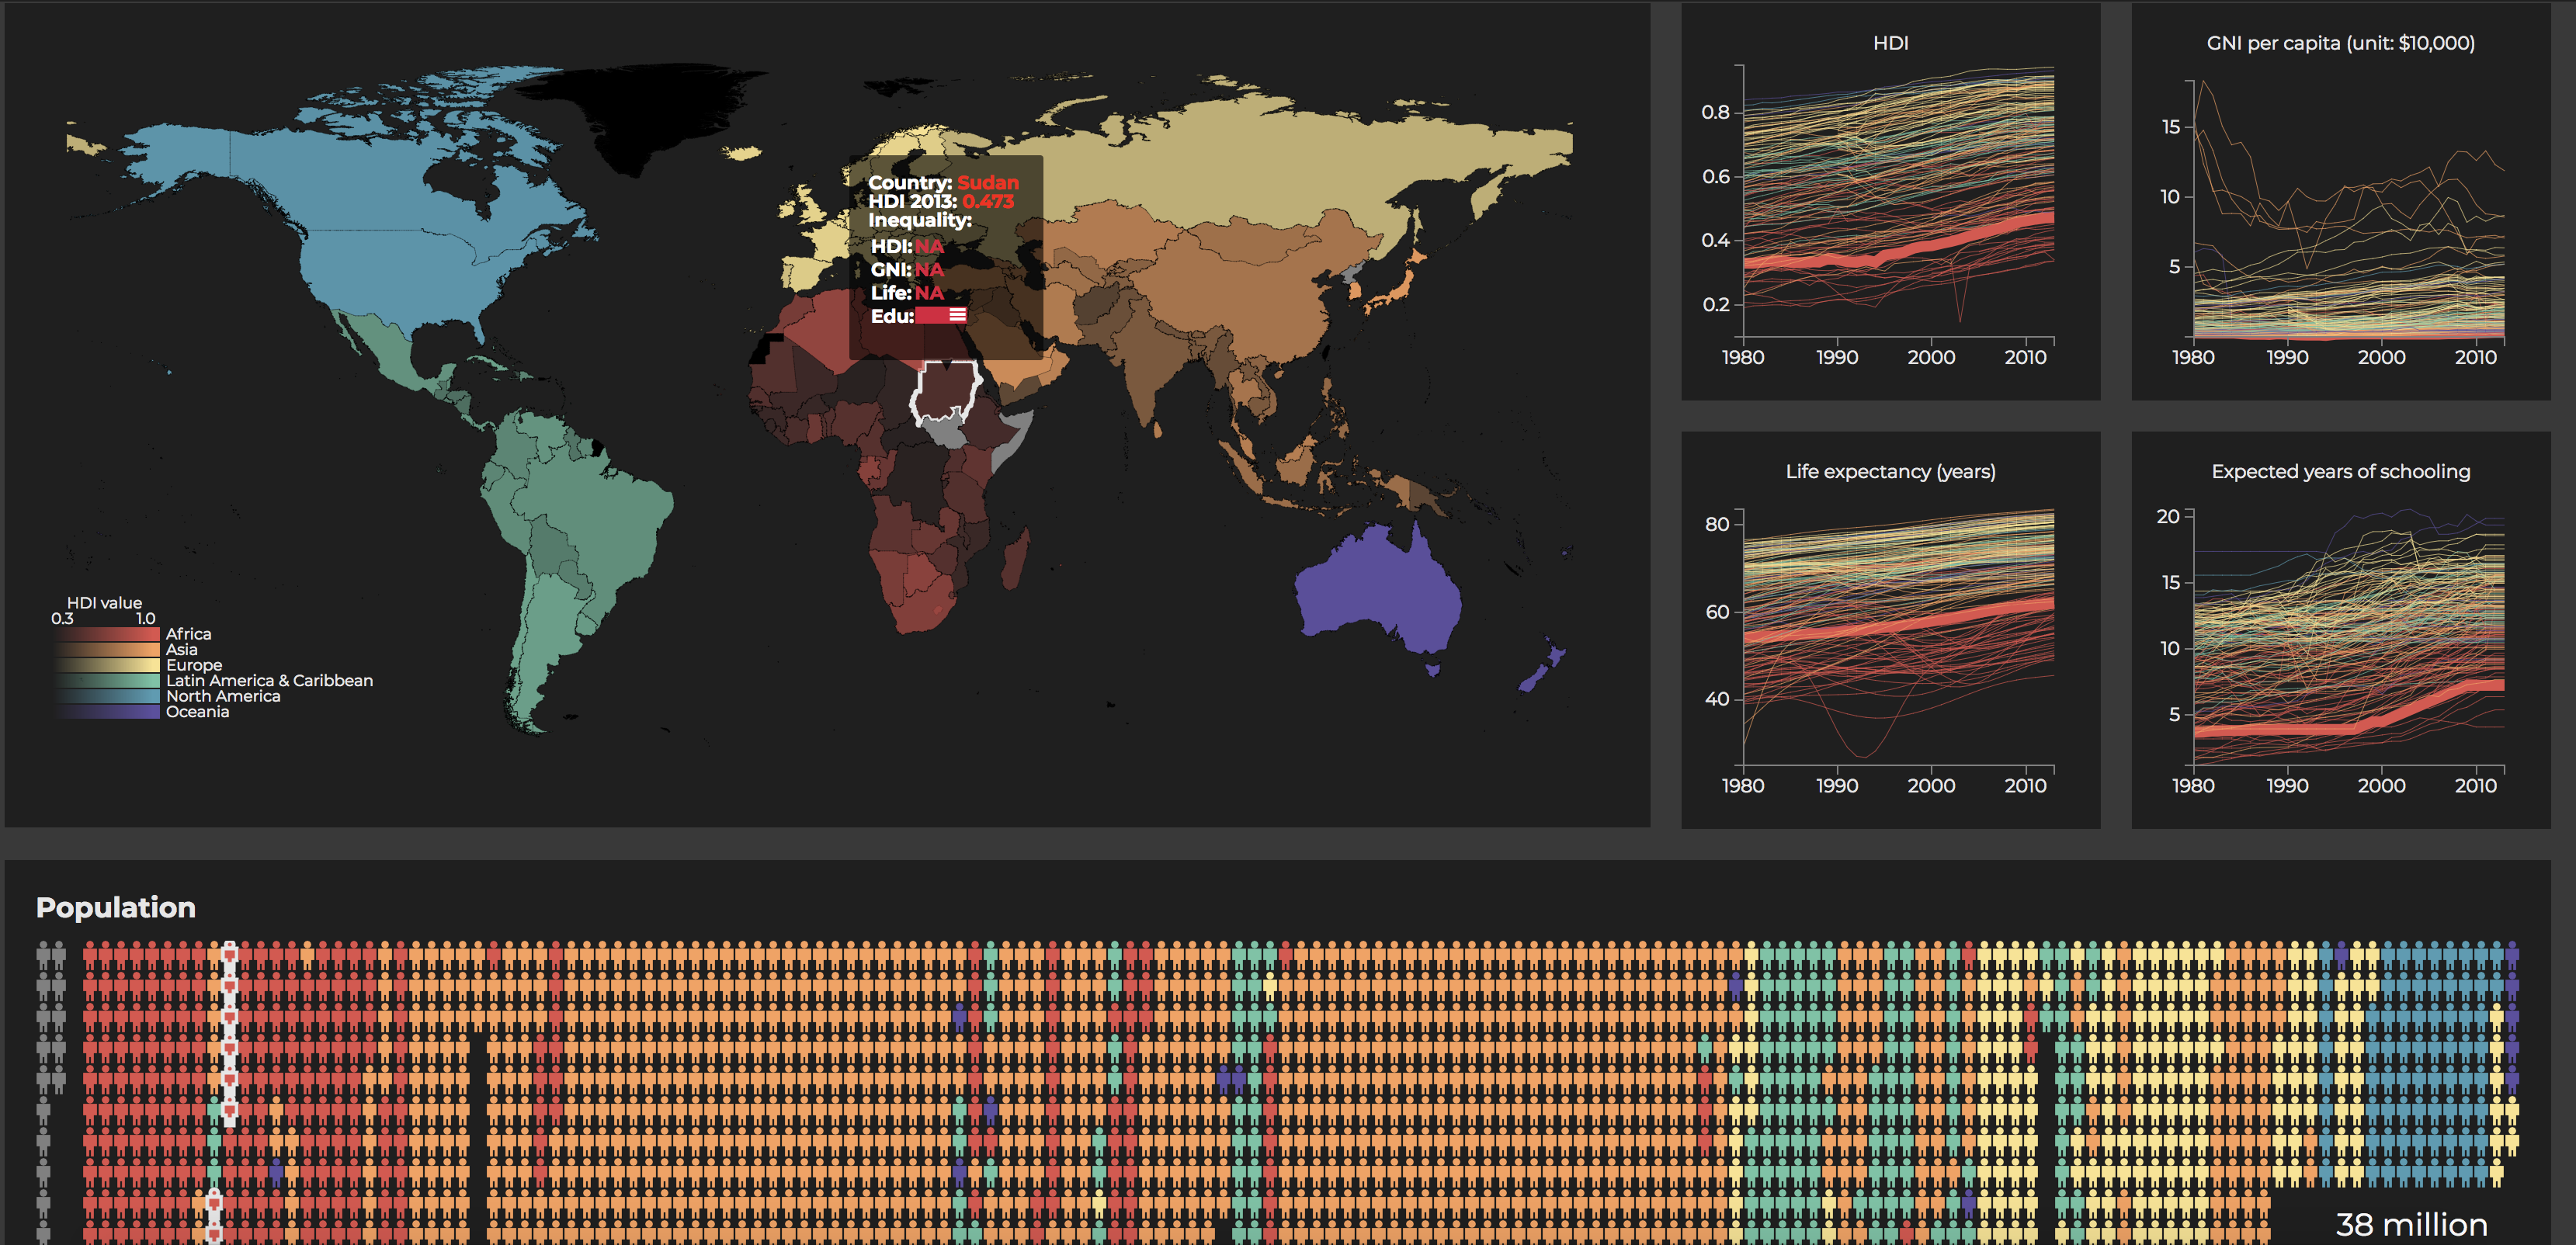
\includegraphics[width=0.4\textwidth]{amazon}
    \caption{Visualizing Human Development Index 2013~\cite{AmazonHDI}}
    \label{fig:amazon}
\end{figure}
